% !TEX root = ../diplomarbeit.tex
\clearpage
\section{Verarbeitung der Spielerpositionen}
\abschnittsautor{E. Akpinar}
\label{sec:umsetzung-akpinar}

Die Auswertung beginnt mit einem Video und einem gespeicherten Feldprofil. Am Ende steht für jede verfolgte Person ein Bericht, der den beobachteten Weg in Metern und die fehlenden Abschnitte ausweist. Entwickelt und untersucht wurde dieser Ablauf an den eigenen Aufnahmen einer einzelnen Kamera. Das Zusammenführen zweier Ansichten ist als späterer Schritt vorgesehen, sobald Spielererkennung und Positionsmessung zusammen ausreichend verlässliche Ergebnisse liefern.

\subsection{Vom kalibrierten Einzelbild zum Videoversuch}
Der folgende Auszug beschreibt den früheren Einzelbildversuch vom Oktober 2026.
\enquote{Die Kalibrierung wird derzeit getrennt vom Tracking anhand des Bilds
\lstinline|kalibrierung_feld.png| durchgeführt. In
\lstinline|punkte.json| werden vier sichtbaren Ecken von Strafraum und
Torraum jeweils Bildkoordinaten und angenommene Feldkoordinaten in Metern
zugeordnet. Daraus berechnet \lstinline|3_homographie.py| die Matrix. Eine gespeicherte Prüfsumme bindet die Kalibrierung an
die verwendete Bilddatei; sie ersetzt jedoch keine Kontrolle der
Punktzuordnung.}~\cite{akpinar-codex-20261029c}

\enquote{Bei der Überprüfung waren drei Bildpunkte den falschen Feldmarkierungen
zugeordnet. Nach dem visuellen Abgleich mit dem Bild wurden die bereits
in \lstinline|referenz.json| hinterlegten Punktzuordnungen übernommen.
Die Kontrollpunkte wurden für diese Korrektur nicht verändert und gehen
nicht in die Berechnung der Matrix ein. Der anschließend neu berechnete
Prüfbericht weist für die drei Kontrollpunkte Positionsabweichungen von
rund 0,66\,m, 0,74\,m und 0,46\,m aus. Für die gespeicherte
Kontrollstrecke ergeben sich 14,97\,m gegenüber einem angenommenen
Referenzwert von 14,62\,m. Die relative Abweichung beträgt rund
2,35\,\%.}~\cite{akpinar-codex-20261029c}

\enquote{Diese Prüfung bezieht sich ausschließlich auf die ausgewählten Punkte
im untersuchten Einzelbild. Die Bildpunkte wurden manuell bestimmt;
die tatsächlichen Abstände auf dem aufgenommenen Spielfeld wurden nicht
unabhängig vermessen. Das Ergebnis ist deshalb eine Plausibilitätsprüfung
unter den gespeicherten Maßannahmen und kein Nachweis der Genauigkeit
von Spielerpositionen oder aufsummierten Laufdistanzen im gesamten Video.}~\cite{akpinar-codex-20261029c}

\subsection{Versuchsfläche und Festlegung der Messpunkte}
Für die Videoauswertung wurde eine zehn Meter lange und zehn Meter breite Fläche mit neun Hütchen markiert. Die jeweils drei Hütchen einer Reihe stehen im Abstand von fünf Metern. Der Abstand wurde sowohl in Querrichtung als auch in Längsrichtung festgelegt. Auch die Lage des mittleren Hütchens wurde beim Aufbau gemessen. Die Bezeichnungen vorne und hinten beziehen sich auf den Blick der Kamera. Beim Anklicken der Punkte bleibt diese Reihenfolge unabhängig davon erhalten, in welche Richtung sich eine Person bewegt.

Für die beiden geraden Versuche wurden zusätzlich zwei vor Ort vorgefundene Gegenstände auf den Boden gelegt. Ihr mit einem Maßband bestimmter Abstand betrug fünf Meter. Beim Gehen und beim Joggen kamen dieselben Start- und Zielmarkierungen zum Einsatz. Bei längeren Strecken wurden andere Markierungen verwendet. Aus der Seitenlänge des Hütchenfeldes lässt sich die Länge eines solchen Laufs deshalb nicht unmittelbar ablesen. Die Videos wurden so geschnitten, dass die für den jeweiligen Lauf relevante Bewegung enthalten ist. Vor dem Start sind keine zusätzlichen Schritte auszuwerten.

Für die Kalibrierung wurde zu jedem Hütchen ein Bildpunkt nahe der Mitte seiner Standfläche gewählt. Diese Wahl ist besonders bei den hinteren Hütchen schwierig. Die Spitze ist oft deutlich zu sehen, liegt jedoch über dem Boden. Der gewählte Bildpunkt muss daher auch bei einer klar erkennbaren Spitze an der unteren Seite des Hütchens angesetzt werden. Der Aufbau verwendet gemessene Abstände, für die Aufstellung und die manuelle Auswahl der Bildpunkte wurde jedoch keine eigene Messunsicherheit bestimmt.

Abb.~\ref{abb:em-feld} zeigt Lage und Funktion der neun Hütchen im Feldmodell.
\begin{figure}[htbp]\centering
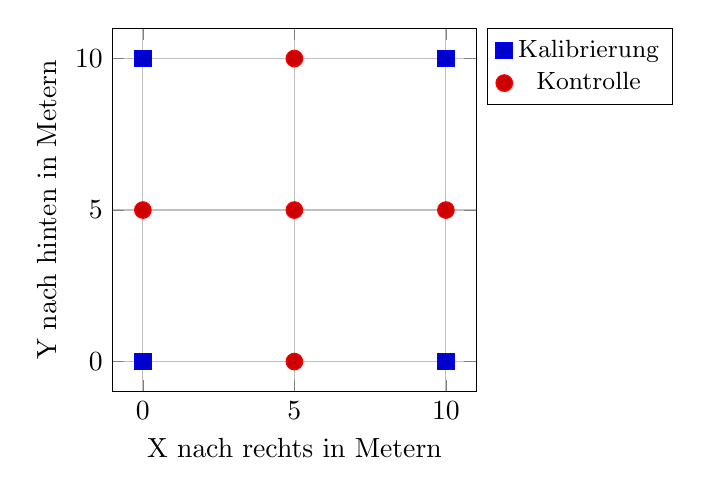
\begin{tikzpicture}\begin{axis}[width=.89\linewidth,height=6.2cm,grid=major,xlabel={X nach rechts in Metern},ylabel={Y nach hinten in Metern},legend style={font=\small},legend pos=north west,axis equal image,xmin=-1,xmax=11,ymin=-1,ymax=11,legend pos=outer north east,xtick={0,5,10},ytick={0,5,10}]
\addplot+[only marks,mark=square*,mark size=3pt] coordinates {(0.000,0.000) (10.000,0.000) (10.000,10.000) (0.000,10.000)};
\addlegendentry{Kalibrierung}
\addplot+[only marks,mark=*,mark size=3pt] coordinates {(5.000,0.000) (0.000,5.000) (5.000,5.000) (10.000,5.000) (5.000,10.000)};
\addlegendentry{Kontrolle}
\end{axis}\end{tikzpicture}
\caption{Lage und Funktion der neun Hütchen im Feldmodell (eigene Darstellung)}\label{abb:em-feld}\end{figure}

\subsection{Referenzprofil und Prüfung der Eingabe}
Ein Profil enthält das Feldmodell, das zugehörige Referenzbild, die vier Punktpaare zur Berechnung und die fünf Kontrollmarkierungen. Jede Markierung hat eine feste Bezeichnung. Dadurch lässt sich im Bericht feststellen, ob etwa die vordere Mitte oder die hintere Mitte Schwierigkeiten verursacht. Bei der Videoauswahl prüft das Programm, ob ein Hütchenprofil vorliegt, ob die neun erwarteten Punkte vorhanden sind und ob das Referenzbild die Größe von $1920\times1080$ Pixeln besitzt. Die nachfolgenden Suchfenster und Abstände in Pixeln beziehen sich auf dieses Bildformat.

Wird ein anderes Video mit demselben Profil ausgewertet, muss ausdrücklich angegeben werden, dass der Hütchenaufbau gleich geblieben ist. Eine solche Bestätigung ist bei einer Serie von Aufnahmen derselben Fläche sinnvoll. Sie gibt lediglich an, welches Modell verwendet werden darf. Ob die Hütchen im aktuellen Bild tatsächlich zu diesem Modell passen, wird weiterhin für jeden Messzeitpunkt geprüft.

Die Kontrollwerte der Referenz lassen sich bereits vor dem ersten Tracking-Schritt untersuchen. Die folgende Tabelle zeigt die Ergebnisse für das Profil aus dem Gehbericht vom 13. November. Sie liefert einen Ausgangswert für die Beurteilung späterer Bilder. Eine Abweichung, die schon in der Referenz vorhanden ist, kann im Video erneut auftreten, auch wenn sich die Kamera kaum bewegt.

Siehe Tab.~\ref{tab:em-referenz}.
\begin{table}[htbp]\centering\caption{Kontrollpunkte des Referenzprofils (eigener Gehbericht vom 13. November)}\label{tab:em-referenz}
\begin{tabular}{@{}llll@{}}\toprule Hütchen & Soll $(X;Y)$ in m & Berechnet $(X;Y)$ in m & Abstand in m\\\midrule
hinten mitte & 5; 10 & 4,83; 10,35 & 0,387\\
mitte links & 0; 5 & -0,06; 4,86 & 0,148\\
mitte mitte & 5; 5 & 4,82; 5,21 & 0,276\\
mitte rechts & 10; 5 & 9,98; 4,85 & 0,155\\
vorne mitte & 5; 0 & 4,78; -0,14 & 0,264\\\bottomrule\end{tabular}\end{table}

\subsection{Videolänge und Auswahl der Messzeitpunkte}
Bei den geschnittenen Aufnahmen können die im Videocontainer eingetragene Bildanzahl und die beim Lesen verfügbare Bildanzahl voneinander abweichen. Für die vollständige Prüfung zählt das Programm mit \lstinline|ffprobe -count_frames| die lesbaren Bilder der ersten Videospur. Aus der Antwort wird \lstinline|nb_read_frames| entnommen. Scheitert die Prüfung oder bricht das Lesen eines zuvor gezählten Bildes ab, wird die Auswertung mit einer Fehlermeldung beendet. Dadurch lässt sich ein abgebrochener Lauf von einer kurzen, aber vollständig gelesenen Aufnahme unterscheiden.

Das Hauptprogramm liest die Bilder in ihrer Reihenfolge und übernimmt für jedes Bild den vom Videoleser gelieferten Zeitstempel. Vor der Weiterverarbeitung prüft es, ob dieser Wert endlich ist und gegenüber dem vorherigen Bild ansteigt. Ein Zeitstempel wird erst dann als regulärer Messzeitpunkt ausgewählt, wenn der nächste Termin erreicht ist. Zusätzlich wird das letzte Bild berücksichtigt. Bei einem Intervall von einer Zehntelsekunde entsteht so ungefähr alle 0,1 Sekunden eine Messung. Der gespeicherte Zeitpunkt kann vom Solltermin geringfügig abweichen.

Beim Hindernisversuch vom 20. November enthält der Bericht 300 als Containerwert angegebene und 297 als lesbar bestätigte Bilder. Der letzte Zeitstempel beträgt rund 4,937 Sekunden. Dass er zwischen zwei regulären Terminen liegt, erklärt den kurzen letzten Abstand der folgenden Auswahl. Für die örtliche Glättung werden die tatsächlichen Zeitunterschiede verwendet.

Siehe Tab.~\ref{tab:em-zeit}.
\begin{table}[htbp]\centering\caption{Auswahl aus der Zeitachse des Hindernisversuchs (eigener Prüfbericht, 15:53 Uhr)}\label{tab:em-zeit}
\begin{tabular}{@{}lll@{}}\toprule Index ab null & Zeit im Video in s & Abstand zum vorigen Messpunkt in s\\\midrule
0 & 0,0000 & Beginn\\
1 & 0,1000 & 0,1000\\
2 & 0,2000 & 0,1000\\
48 & 4,8033 & 0,1017\\
49 & 4,9033 & 0,1000\\
50 & 4,9367 & 0,0333\\\bottomrule\end{tabular}\end{table}

\subsection{Nachführung bei kleinen Änderungen der Kameraansicht}
Bleibt das Feld stehen, kann sich seine Lage im Bild trotzdem ändern. Eine einmal markierte Ecke würde dann an der alten Bildstelle gesucht. Die Nachführung bestimmt zuerst die Bewegung zwischen Referenzbild und aktuellem Bild. Als Anhaltspunkte dienen wiedererkennbare Helligkeitsmuster aus der Umgebung des vermessenen Bodens. Bereiche erkannter Personen werden aus der Suche ausgeblendet, weil eine mitlaufende Jacke keine Auskunft über die Lage des Feldes gibt.

Für die Suche verwendet die Klasse \lstinline|KameraNachfuehrung| das ORB-Verfahren (Oriented FAST and Rotated BRIEF) aus OpenCV. Zu einem Merkmal werden die zwei ähnlichsten Kandidaten gesucht. Der beste Kandidat muss einen deutlich kleineren Abstand als der zweitbeste aufweisen. Treffen mehrere Referenzpunkte denselben Punkt im neuen Bild, wird nur die beste Zuordnung behalten. Erst bei mindestens zwanzig eindeutigen Treffern wird eine mögliche Bildtransformation berechnet.

RANSAC (Random Sample Consensus) sucht eine Transformation, zu der möglichst viele der gefundenen Paare passen. Für die Freigabe werden anschließend die Zahl der passenden Paare, ihr Anteil, ihre räumliche Verteilung und der verbleibende Bildfehler geprüft. Eine Ansammlung ähnlicher Merkmale an nur einer Stelle der Aufnahme reicht daher für sich genommen nicht aus. Das Verfahren kann ausdrücklich eine unsichere Kamerazuordnung zurückgeben. Für das betreffende Bild fehlt dann die Grundlage zur Messung auf dem Feld.

Siehe Tab.~\ref{tab:em-kamera}.
\begin{table}[htbp]\centering\caption{Prüfbedingungen der Kameranachführung (eigene Implementierung)}\label{tab:em-kamera}
\begin{tabular}{@{}ll@{}}\toprule Prüfgröße & Bedingung\\\midrule
Eindeutige Treffer vor der Schätzung & mindestens 20\\
Treffer passend zur Transformation & mindestens 12\\
Anteil passender Treffer & mindestens 55 Prozent\\
Flächenanteil der passenden Merkmale & mindestens 15 Prozent\\
Median des Bildfehlers & höchstens 2 Pixel im verkleinerten Bild\\\bottomrule\end{tabular}\end{table}

\subsection{Lokale Suche an den neun Hütchen}
Die geschätzte Kamerabewegung gibt für jedes Hütchen eine neue Suchposition vor. Zur genaueren Prüfung wird das aktuelle Graubild zunächst in die Ansicht der Referenz zurückgerechnet. Um den ursprünglich gewählten Bodenpunkt liegt ein kleiner Bildausschnitt. Er reicht weiter nach oben als nach unten und enthält dadurch einen Teil des Hütchenkörpers. In der ausgerichteten Aufnahme sucht das Programm die Position, an der dieser Ausschnitt am besten passt. Aus der Verschiebung des Musters folgt die neue Lage des markierten Bodenpunkts.

Ein gutes Ergebnis des Bildvergleichs allein genügt nicht. Ein Muster am Rand des Suchbereichs könnte beispielsweise nur deshalb der beste Treffer sein, weil die richtige Stelle außerhalb liegt. Auch Bildflächen, die durch das Zurückrechnen über den Bildrand geraten sind, dürfen keinen regulären Treffer liefern. Das Programm führt solche Gründe je Hütchen getrennt auf. Bei einem schlecht sichtbaren Punkt kann somit später nachvollzogen werden, weshalb er aus der Kontrolle herausgenommen wurde.

Zusätzlich wird geprüft, ob sich der gefundene oder der erwartete Punkt innerhalb eines Personenkastens befindet. Beide Stellen sind relevant. Verdeckt ein Spieler das Hütchen, kann die Mustersuche knapp neben ihm einen ähnlich aussehenden Gegenstand finden. Eine Prüfung allein an der gefundenen Stelle würde den verdeckten Sollort übersehen. Umgekehrt kann ein falsch erkannter Personenkasten einen sichtbaren Kontrollpunkt sperren. Der Zusammenhang zwischen Erkennung und Feldmessung entsteht hier schon vor der eigentlichen Berechnung einer Spielerposition.

Siehe Tab.~\ref{tab:em-suche}.
\begin{table}[htbp]\centering\caption{Arbeitswerte der lokalen Hütchensuche im Referenzformat (eigener Programmstand)}\label{tab:em-suche}
\begin{tabular}{@{}ll@{}}\toprule Größe & Wert oder Entscheidung\\\midrule
Muster um den Bildpunkt & bis zu 31 Pixel breit und 54 Pixel hoch\\
Zusätzlicher lokaler Suchraum & 20 Pixel je Richtung vor Begrenzung\\
Verwertbare Fläche des Ausschnitts & mindestens 98 Prozent\\
Ähnlichkeitswert & mindestens 0,65\\
Abstand zur erwarteten Position & höchstens 25 Pixel\\
Treffer am äußeren Suchrand & gesonderter Ablehnungsgrund\\\bottomrule\end{tabular}\end{table}

\subsection{Feldübertragung bei einer verdeckten Ecke}
Sind die vier äußeren Hütchen brauchbar, wird die Umrechnung aus ihren aktuellen Bildpositionen neu berechnet. Fällt eine Ecke aus, steht ein zweiter Weg zur Verfügung. Dazu wird die Kalibrierung der Referenz mit der gültigen Kamerabewegung kombiniert. Bezeichnet $B$ die Abbildung von der Referenz in das aktuelle Bild und $H_R$ die Umrechnung aus dem Referenzbild in Meter, so gilt für das aktuelle Bild
\[
H_{\mathrm{aktuell}}=H_R B^{-1}.
\]
Die Reihenfolge folgt aus dem Weg des Bildpunktes. Zuerst gelangt er zurück in die Referenz, anschließend in den Feldplan. Das Verfahren bezieht sich in jedem Bild auf dieselbe Referenz. Dadurch muss die Verschiebung einer früher geschätzten Ecke nicht in alle folgenden Bilder übernommen werden.

Eine solche Übertragung wird nur bei mindestens drei verwendbaren Kontrollhütchen zugelassen. Diese müssen eine ausreichend große Fläche aufspannen. Drei Punkte auf einer Linie liefern selbst dann keine Fläche, wenn jeder einzelne im Bild gut sichtbar ist. Beim zehn mal zehn Meter großen Feld entsprechen die geforderten 15 Prozent einer Fläche von 15 Quadratmetern. Zusätzlich werden alle noch sichtbaren Ecken und Kontrollpunkte mit den zugehörigen Feldpositionen verglichen. Der größte zugelassene Abstand beträgt 0,5 Meter.

Im Prüfbericht kennzeichnet \lstinline|geometry_method| die Entscheidung. Eine übertragene Ecke beschreibt die Lage, die aus der gültigen Referenz folgen würde. Für die spätere Auswertung bleibt damit erkennbar, auf welcher Grundlage die Freigabe erfolgt ist. Auch nach einer Freigabe kann die Personenposition aus anderen Gründen fehlen.

\subsection{Bodenpunkt und gleichzeitige Verarbeitung mehrerer Personen}
Das Auswertungsprogramm lädt im untersuchten Stand die lokale Datei \lstinline|yolov8n.pt|. Die Klassen werden anhand der Bezeichnungen des geladenen Modells ausgewählt. Als Personenklassen berücksichtigt die Implementierung die Namen person, player, goalkeeper und referee. Ein erkannter Ball kann daher im projektbezogenen Modell eine andere Nummer als ein Spieler tragen, ohne als Laufspur übernommen zu werden. Das getrennte Skript \lstinline|test_tracking.py| erlaubt die Auswahl einer anderen Modelldatei für Vergleiche.

Für einen Kasten mit den horizontalen Grenzen $u_l$ und $u_r$ sowie der Unterkante $v_u$ lautet der verwendete Bildpunkt $((u_l+u_r)/2,v_u)$. Anschließend wird geprüft, ob er innerhalb des Feldvierecks liegt. Im ersten ausgewerteten Bild des Gehversuchs reicht der Kasten horizontal von ungefähr 682 bis 751 Pixeln. Die Mitte liegt bei rund 717 Pixeln, die Unterkante bei rund 780 Pixeln. Die Rechenregel ist somit bereits am gespeicherten Kasten nachvollziehbar. Wie gut dieser Punkt dem tatsächlichen Standpunkt entspricht, hängt vom Bild ab.

Zu jedem Zeitpunkt wird eine Liste der Personen geführt. Enthält das Bild zwei Personen mit verschiedenen Kennnummern, entstehen zwei Positionsdatensätze mit demselben Zeitstempel. Fehlt die Nummer oder wird sie im Feld doppelt verwendet, ist die Zuordnung für den betreffenden Kandidaten uneindeutig. Eine andere Person mit eindeutiger Nummer kann weiterhin berücksichtigt werden. Erst nach dieser Auswahl und einer gültigen Feldprüfung werden die Bildkoordinaten in Meter umgerechnet.

Siehe Tab.~\ref{tab:em-ballreihe}.
\begin{table}[htbp]\centering\caption{Zwei unabhängige Positionen zur selben Zeit (eigener Ballwurfbericht vom 16. November)}\label{tab:em-ballreihe}
\begin{tabular}{@{}llll@{}}\toprule Zeit in s & Spur & X in m & Y in m\\\midrule
0,0 & 1 & 7,47 & 2,86\\
0,0 & 2 & 2,46 & 2,88\\
1,5 & 1 & 7,52 & 2,94\\
1,5 & 2 & 2,55 & 2,97\\
3,0 & 1 & 7,61 & 2,31\\
3,0 & 2 & 2,57 & 2,86\\\bottomrule\end{tabular}\end{table}

\subsection{Spurfortsetzung nach einer Verdeckung}
Beim dichten Tracking wird jedes gelesene Bild an BoT-SORT übergeben. Die Ausgabe der Meterpositionen behält ihren eigenen Takt. Die größere Anzahl von Zwischenbildern soll dem Tracker auch bei einer Begegnung die zeitliche Zuordnung erleichtern. Gleichzeitig ändert die Option im heutigen Programm die Größe der Eingabe von 640 auf 960, die Erkennungsschwelle von 0,25 auf 0,1 und den Zuordnungsparameter der Tracker-Konfiguration. Ein Vergleich der beiden Betriebsarten untersucht deshalb mehrere Änderungen zusammen.

Für die nachträgliche Prüfung einer möglichen Fortsetzung betrachtet das Programm das Ende einer Spur und den Beginn einer anderen. Zwischen beiden muss eine kurze Lücke liegen. Die Zeit muss ansteigen, die Feldzuordnung muss durchgehend gültig sein und der Ortswechsel muss innerhalb der Sprunggrenze liegen. Zusätzlich wird eine andere Spur gesucht, die vor, während und nach der Lücke sichtbar ist und als verdeckende Person in Frage kommt. Eine beliebige Pause zwischen zwei ähnlich aussehenden Spielern genügt damit nicht.

Auch die Farbe am Oberkörper wird vor und nach der Begegnung verglichen. Liegen genügend verwertbare Farbproben vor und sind beide Enden einander eindeutig zuzuordnen, kann die neue Spur derselben Auswertungsnummer zugewiesen werden. Die vom Tracker ursprünglich vergebene Nummer bleibt im Datensatz erhalten. Bei gleichfarbigen Trikots liefert das Farbmerkmal wenig Unterscheidungskraft. Die Zuordnung bleibt eine begründete Annahme und muss sich am Video prüfen lassen.

Ein weiterer Schritt behandelt den Bodenpunkt unabhängig von der Kennnummer. Überlappt der untere Teil des Kastens ausreichend mit einer weiter vorne erkannten Person, wird der Fußpunkt als möglicherweise verdeckt geführt. Die verworfenen Einträge werden getrennt gespeichert. So lässt sich im Nachhinein unterscheiden, ob die Person ganz verschwunden ist oder ob nur ihre Füße für eine Meterposition nicht sichtbar genug waren.

\subsection{Bildung von Teilstrecken und Ausgabe der Ergebnisse}
Für jede Person wird die gemeinsame Zeitachse des Videos durchlaufen. Eine gültige Folge endet bei einer fehlenden Position, einem Wechsel der Kennnummer, einem zu großen Zeitabstand oder einem unplausiblen Sprung. Als vorläufige Grenzen gelten das 1,6-Fache des eingestellten Messintervalls und zwölf Meter pro Sekunde. Liegt nur ein einzelner Punkt vor, lässt sich daraus keine Teilstrecke bilden.

Innerhalb einer gültigen Folge wird um jeden Messzeitpunkt eine lokale Gerade an die benachbarten Positionen angepasst. Bei einem Intervall von 0,1 Sekunden werden regulär fünf Werte herangezogen. Am Rand wird das Fenster in den verfügbaren Abschnitt verschoben. Aus der geglätteten Folge wird ein neuer Wegpunkt erst gezählt, wenn sein Abstand zum letzten gezählten Punkt mindestens zehn Zentimeter beträgt. Kleinere aufeinanderfolgende Bewegungen können den Abstand zum selben Bezugspunkt allmählich vergrößern. Der Bezugspunkt wechselt erst, wenn die Schwelle erreicht ist.

Die Positionstabelle enthält die übernommenen Meterpositionen. Die separate Tabelle der Laufwegpunkte enthält zusätzlich Rohkoordinaten, geglättete Koordinaten, den gezählten Schritt und die bisherige Summe innerhalb des Abschnitts. Im Prüfbericht bleiben die Kamerabewegung, Ablehnungsgründe und der Bezug zum Kontrollbild erhalten. Der Bericht kann damit sowohl zur Sichtprüfung einer fraglichen Stelle als auch zur Nachrechnung einer Strecke verwendet werden. Die lokale HTML-Übersicht stellt diese Daten nach Spur und Zeitpunkt dar.

Für kurze, plausibel verdeckte Abschnitte kann eine zusätzliche geradlinige Schätzung zwischen den geprüften Endpunkten erstellt werden. Die Zwischenwerte richten sich nach der Videozeit. Die Wegbilanz weist beobachtete und geschätzte Meter gesondert aus. Ein offener Zeitabschnitt darf bei der Auswertung nicht als Stillstand interpretiert werden.

\subsection{Vom einzelnen Bildtreffer zum gezählten Wegpunkt}
Wie sich die Entscheidungen im Programm auswirken, lässt sich am Beginn des Gehversuchs nachvollziehen. Zu jedem Zeitstempel liegen zunächst die beiden Rohkoordinaten in Metern vor. Die örtliche Glättung liefert ein zweites Koordinatenpaar. Für die Wegsumme wird anschließend nur die Entfernung vom letzten gezählten Bezugspunkt berücksichtigt. Haben zwei benachbarte Zeilen denselben Summenwert, bedeutet das somit nicht zwangsläufig, dass beide Positionen identisch sind.

Die Tabelle zeigt die ersten acht aufeinanderfolgenden Einträge. Die Spalte Schritt gibt den tatsächlich zur Wegsumme addierten Betrag an. Alle Werte sind für die Darstellung gerundet. Die Entscheidung an der Zehn-Zentimeter-Grenze wurde im Programm mit den ungerundeten Koordinaten getroffen.

Siehe Tab.~\ref{tab:em-punkte}.
\begin{table}[htbp]\centering\caption{Erste Wegpunkte des Gehversuchs (eigene Laufwegtabelle vom 13. November)}\label{tab:em-punkte}
\begin{tabular}{@{}llllll@{}}\toprule Zeit in s & X roh in m & Y roh in m & X glatt in m & Y glatt in m & Schritt in m\\\midrule
0,00 & 2,208 & 3,693 & 2,210 & 3,705 & 0,000\\
0,10 & 2,220 & 3,766 & 2,227 & 3,683 & 0,000\\
0,20 & 2,259 & 3,581 & 2,245 & 3,660 & 0,000\\
0,30 & 2,265 & 3,596 & 2,260 & 3,655 & 0,000\\
0,40 & 2,274 & 3,664 & 2,281 & 3,629 & 0,105\\
0,50 & 2,283 & 3,669 & 2,302 & 3,665 & 0,000\\
0,60 & 2,325 & 3,632 & 2,336 & 3,720 & 0,106\\
0,70 & 2,363 & 3,766 & 2,377 & 3,753 & 0,000\\\bottomrule\end{tabular}\end{table}

Abb.~\ref{abb:em-tiefegang} zeigt Rohposition und geglättete Position in Feldtiefe während des Gehversuchs.
\begin{figure}[htbp]\centering
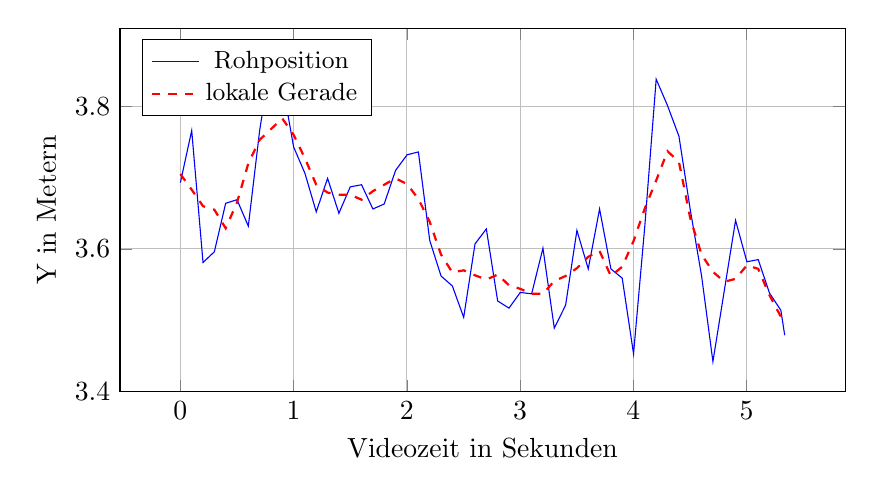
\begin{tikzpicture}\begin{axis}[width=.89\linewidth,height=6.2cm,grid=major,xlabel={Videozeit in Sekunden},ylabel={Y in Metern},legend style={font=\small},legend pos=north west,]
\addplot+[thin,mark=none] coordinates {(0.000,3.693) (0.100,3.766) (0.200,3.581) (0.300,3.596) (0.400,3.664) (0.500,3.669) (0.600,3.632) (0.700,3.766) (0.800,3.867) (0.900,3.833) (1.000,3.743) (1.100,3.706) (1.200,3.652) (1.300,3.699) (1.400,3.650) (1.500,3.687) (1.600,3.690) (1.700,3.656) (1.800,3.663) (1.900,3.710) (2.002,3.732) (2.102,3.736) (2.202,3.612) (2.302,3.562) (2.402,3.548) (2.502,3.504) (2.602,3.607) (2.702,3.628) (2.802,3.527) (2.902,3.517) (3.002,3.539) (3.102,3.537) (3.202,3.601) (3.302,3.489) (3.402,3.521) (3.502,3.626) (3.602,3.572) (3.702,3.656) (3.802,3.572) (3.902,3.559) (4.002,3.453) (4.102,3.633) (4.202,3.838) (4.302,3.801) (4.403,3.758) (4.503,3.655) (4.603,3.562) (4.703,3.442) (4.803,3.541) (4.903,3.640) (5.003,3.582) (5.103,3.585) (5.203,3.538) (5.303,3.514) (5.337,3.479)};
\addlegendentry{Rohposition}
\addplot+[thick,dashed,mark=none] coordinates {(0.000,3.705) (0.100,3.683) (0.200,3.660) (0.300,3.655) (0.400,3.629) (0.500,3.665) (0.600,3.720) (0.700,3.753) (0.800,3.768) (0.900,3.783) (1.000,3.760) (1.100,3.727) (1.200,3.690) (1.300,3.679) (1.400,3.676) (1.500,3.676) (1.600,3.669) (1.700,3.681) (1.800,3.690) (1.900,3.699) (2.002,3.691) (2.102,3.670) (2.202,3.638) (2.302,3.592) (2.402,3.567) (2.502,3.570) (2.602,3.563) (2.702,3.557) (2.802,3.564) (2.902,3.549) (3.002,3.544) (3.102,3.537) (3.202,3.537) (3.302,3.555) (3.402,3.562) (3.502,3.573) (3.602,3.589) (3.702,3.597) (3.802,3.562) (3.902,3.575) (4.002,3.611) (4.102,3.657) (4.202,3.696) (4.302,3.737) (4.403,3.722) (4.503,3.643) (4.603,3.592) (4.703,3.568) (4.803,3.554) (4.903,3.558) (5.003,3.577) (5.103,3.572) (5.203,3.535) (5.303,3.505) (5.337,3.495)};
\addlegendentry{lokale Gerade}
\end{axis}\end{tikzpicture}
\caption{Rohposition und geglättete Position in Feldtiefe während des Gehversuchs (eigene Darstellung)}\label{abb:em-tiefegang}\end{figure}
Die beiden Linien stellen dieselbe Aufnahme und dieselbe Person dar. Ihre Differenz zeigt, wie stark die lokale Anpassung den gemessenen Verlauf verändert. Ob eine einzelne seitliche oder vorwärts gerichtete Bewegung vom Spieler stammt, lässt sich daraus allein nicht entscheiden. Dafür bleibt das Kontrollbild zum betreffenden Zeitpunkt erforderlich.


\subsection{Geradlinige Schätzung an einer konkreten Verdeckung}
Im Hindernisbericht vom 20. November lässt sich die Berechnung an Spur 2 Schritt für Schritt zurückverfolgen. Bei etwa 1,40 Sekunden endet ein beobachteter Abschnitt bei $(1{,}467;3{,}939)$ Metern. Der verwendete Anfang des folgenden Abschnitts liegt bei 2,10 Sekunden und $(2{,}430;4{,}334)$ Metern. Die Komponenten der Verschiebung betragen damit rund 0,963 und 0,395 Meter. Der direkte Abstand der beiden Endpunkte ergibt rund 1,040 Meter.

Für einen Zeitpunkt $t$ zwischen den beiden Enden wird der bereits verstrichene Anteil der Lücke berechnet. Bei 1,50 Sekunden sind etwa 0,10 von 0,70 Sekunden vergangen. Die erste geschätzte Position liegt daher ungefähr ein Siebtel des Wegs vom letzten sichtbaren zum nächsten sichtbaren Punkt entfernt. Dieses Vorgehen setzt eine gleichförmige Bewegung entlang der Verbindung voraus. Tatsächlich könnte die Person hinter dem Hindernis kurz gebremst oder ihre Richtung geändert haben.

Die Tabelle enthält die vom Bericht gespeicherten Zwischenwerte dieser einen Lücke. Ihre regelmäßige Anordnung ergibt sich aus der Rechenvorschrift. Sie liefert keine zusätzlichen Beobachtungen des Spielers. Deshalb werden solche Punkte in der Wegbilanz der geschätzten Strecke zugerechnet.

Siehe Tab.~\ref{tab:em-interpol}.
\begin{table}[htbp]\centering\caption{Zeitliche Verteilung der geschätzten Punkte für Spur 2 (eigener Bericht, 15:53 Uhr)}\label{tab:em-interpol}
\begin{tabular}{@{}llll@{}}\toprule Zeit in s & X in m & Y in m & Grundlage\\\midrule
1,40 & 1,467 & 3,939 & sichtbarer Endpunkt\\
1,50 & 1,605 & 3,995 & geschätzt\\
1,60 & 1,742 & 4,052 & geschätzt\\
1,70 & 1,880 & 4,108 & geschätzt\\
1,80 & 2,017 & 4,165 & geschätzt\\
1,90 & 2,155 & 4,221 & geschätzt\\
2,00 & 2,292 & 4,278 & geschätzt\\
2,10 & 2,430 & 4,334 & sichtbarer Anfangspunkt\\\bottomrule\end{tabular}\end{table}
Im selben Bericht ordnet das Programm die ursprünglichen Tracker-Nummern 14, 21 und 23 der Auswertungsnummer 2 zu. Diese Zuordnung beschreibt die Entscheidung des Programms. Für eine Prüfung der tatsächlichen Identität sind an jedem Übergang die beiden benachbarten Kontrollbilder und die übrigen sichtbaren Personen heranzuziehen. Die rechnerisch passende Verbindung ist dafür nur ein Anhaltspunkt.
\clearpage
